\chapter{Návrh}

\section{Návrh způsobu specifikace pravidel}

Abychom mohli specifikovat pravidla, musíme nejprve definovat strukturu, nad kterou budou tato pravidla platit. V tomto textu formalizujeme model programu pomocí teorie grafů. Nad grafem je možné dále specifikovat pravidla, která musí vstupní projekt splňovat.

\subsection{Formalizace modelu programu pomocí grafu}
\label{design-graph_formalization}

Analyzovaný softwarový projekt abstrahujeme jako orientovaný multigraf rozšířený o zobrazení množiny uzlů do množiny typů a zobrazení hran do množiny jejich klasifikátorů (označení typu vztahu mezi uzly). Dále přidáme ke každému vrcholu zobrazení, které mu přiřadí jméno (řetězec). Získáme tak následující strukturu:

\begin{displaymath}
  G = \langle V, E, \rho, K, C, N, \mathit{Kind}, \mathit{Class}, \mathit{Name}\rangle
  \label{extended_multigraph}
\end{displaymath}
v níž platí:
\begin{itemize}
\item $V$ je množina elementů (v našem případě části kódu)
\item $E$ je množina hran (v našem případě vztahy mezi částmi kódu - např. volání funkce, dědičnost)
\item $V \cap E = \emptyset$
\item $\rho: E \mapsto V \times V$ je zobrazení množiny hran do množiny uspořádaných dvojic vrcholů (incidence)
\item $K$ je libovolná množina označení typů vrcholů\footnote{Pod pojmem typ zde rozumíme jakékoliv označení, které specifikuje o jaký objekt se jedná -- může to být třída, metoda, příkaz, \ldots},
\item $\mathit{Kind}: V \mapsto K$ je zobrazení, které přiřadí každému vrcholu jeho typ,
\item $C$ je množina klasifikátorů hran,
\item $N$ je množina jmen (řetězců)
\item $\mathit{Class}: E \mapsto C$ je zobrazení, které přiřadí každé hraně její klasifikátor (zda se jedná o \emph{method call}, \emph{dědičnost}, atd.)
\item $\mathit{Name}: V \mapsto N$ je zobrazení, které přiřadí vrcholu jeho jméno (např. jméno třídy, jméno metody, \ldots)
\end{itemize}

Ukázka formalizace zdrojového kódu pomocí grafu je na obrázku \ref{design-graph_example}. V uvedeném příkladě můžeme strukturu $G$ namapovat následujícím způsobem:
\begin{figure}[h!]
  \centering
  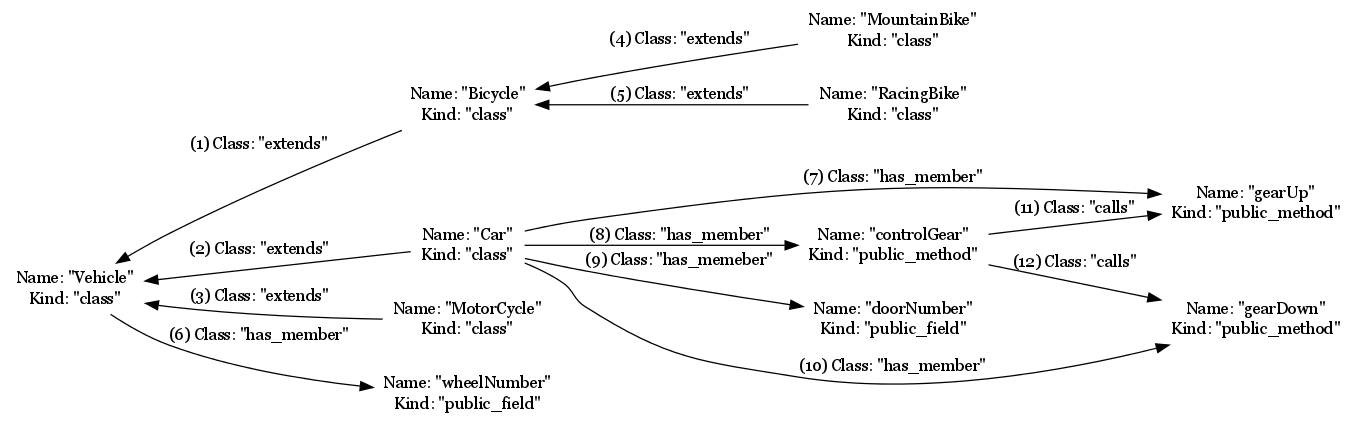
\includegraphics[width=1.0\textwidth]{./graphs/graph_example.png}
  \caption{Příklad formalizace hierarchie tříd jako grafu.\label{design-graph_example}}
\end{figure}
Množinu vrcholů můžeme ztotožnit s množinou názvů elementů (v našem případě třídy, pole, metody)\footnote{V konečném důsledku bude tato množina představována konkrétními elementy tak, jak se nalézají ve zdrojovém kódu.}.
\begin{align*}
  V = &\{ \\
  &Vehicle, Car, MotorCycle, Bicycle, MountainBike, RacingBike, \\
  &wheelNumber, doorNumber, \\
  &controlGear, gearUp, gearDown \\
  &\}
\end{align*}
Abychom mohli demonstrovat množinu hran, bylo provedeno očíslování. Hranu zde identifikujeme číslem. V počítačové reprezentaci se může jednat o konkrétní objekt uložený v poli. Množinu hran potom můžeme reprezentovat prostým výčtem čísel:
\begin{displaymath}
  E = \{1, 2, 3, 4, 5, 6, 7, 8, 9, 10, 11, 12\}
\end{displaymath}
Zobrazení $\rho$ můžeme formálně zapsat jako následující množinu\footnote{Zobrazení je binární relace. Proto jej můžeme reprezentovat jako množinu uspořádaných dvojic.}:
\begin{align*}
  \rho = &\{ \\
  &(1, (Bicycle, Vehicle)), \\
  &(2, (Car, Vehicle)), \\
  &(3, (MotorCycle, Vehicle)), \\
  &(4, (MountainBike, Bicycle)), \\
  &(5, (RacingBike, Bicycle)), \\
  &(6, (Vehicle, wheelNumber)), \\
  &(7, (Car, gearUp)), \\
  &(8, Car, controlGear)), \\
  &(9, (Car, doorNumber)), \\
  &(10, (Car, gearDown)), \\
  &(11, (controlGear, gearUp)), \\
  &(12, (controlGear, gearDown)) \\
  &\}
\end{align*}
Zbývají nám množina typů $K$,
\begin{align*}
  K = \{ class, public\_field, public\_method \}
\end{align*}
množina klasifikátorů hran $C$,
\begin{align*}
  C = \{ \langle\langle{}extends\rangle\rangle, \langle\langle{}has\_member\rangle\rangle, \langle\langle{}calls\rangle\rangle \}
\end{align*}
přiřazení typů uzlům $Kind$,
\begin{align*}
  Kind = &\{ \\
  &(Bicycle, class), \\
  &(Car, class), \\
  &(MotorCycle, class), \\
  &(MountainBike, class), \\
  &(RacingBike, class), \\
  &(Vehicle, class), \\
  &(wheelNumber, public\_field), \\
  &(doorNumber, public\_field), \\
  &(controlGear, public\_method), \\
  &(gearUp, public\_method), \\
  &(gearDown, public\_method) \\
  &\}
\end{align*}
a přiřazení klasifikátorů hranám:
\begin{align*}
  Class = &\{ \\
  &(1, \langle\langle{}extends\rangle\rangle), \\
  &(2, \langle\langle{}extends\rangle\rangle), \\
  &(3, \langle\langle{}extends\rangle\rangle), \\
  &(4, \langle\langle{}extends\rangle\rangle), \\
  &(5, \langle\langle{}extends\rangle\rangle), \\
  &(6, \langle\langle{}has\_member\rangle\rangle), \\
  &(7, \langle\langle{}has\_member\rangle\rangle), \\
  &(8, \langle\langle{}has\_member\rangle\rangle), \\
  &(9, \langle\langle{}has\_memeber\rangle\rangle), \\
  &(10, \langle\langle{}has\_member\rangle\rangle), \\
  &(11, \langle\langle{}calls\rangle\rangle), \\
  &(12, \langle\langle{}calls\rangle\rangle), \\
  \}
\end{align*}

%% Graf elementů použitých v kódu. Vrcholy $v \in V$ představují různé syntaktické elementy v analyzovaném kódu. Záleží na úrovni prováděné analýzy, jaké zvolíme vrcholy. V případě, že budeme analyzovat \uv{nízkoúrovňové} chování funkce, mohou být vrcholy jednotlivé příkazy a jejich části. Pokud budeme analyzovat míru provázanosti tříd nebo metod, stačí když použijeme jako vrcholy třídy a metody (případně parametry metod.)
%% $G = (V, E)$

\subsection{Formalizace pravidel}

Nyní, když máme definován model, můžeme popsat jazyk pravidel, která mají pro daný model platit. Vytvoříme jednoduchý jazyk (DSL) pro specifikaci validačních parametrů. Jazyk popíšeme jednoduchou gramatikou (listing \ref{design-grammar}). U této gramatiky předpokládáme, že bílé znaky jsou ignorovány (pokud nejsou uvnitř řetězce).

TODO: definovat základní elementy jazyka pravidel

\begin{itemize}
\item co jsou to selektory (napsat definici platnou pro tento dokument),
\item co jsou to predikáty (napsat definici platnou pro tento dokument),
\item popis základní struktury souboru s definicí validačních pravidel,
\item ukázka dokumentu odpovídajícího specifikované gramatice.
\end{itemize}

%% TODO: zde gramatika nebude - již je vložena v příloze -- do práce ji zahrneme, protože je to důležitá část dokumentaci (udává přesný formát, který může použít uživatel při specifikaci pravidel)
%% TODO: na tomto místě popsat formát pravidel matematicky

%% TODO: přepsat jako přesné definice, které se budou v dalším textu dodržovat
\subsubsection{Typy operátorů}
\begin{itemize}
\item Predikát (Predicate) -- operátor, který na základě vstupních parametrů a poskytované rozhodovací funkce vrací booleovskou hodnotu (true/false)
\item Vrcholový selektor (Vertex selector) -- vrací množinu vrcholů na základě vstupních parametrů a poskytované výběrové funkce
\item Hranový selector (Edge selector) -- vrací množinu hran na základě vstupních parametrů a poskytované výběrové funkce
\end{itemize}

\lstset{
    basicstyle=\ttfamily,
    numbers=left,
    numberstyle=\footnotesize,
    commentstyle=\color{gray}\textit,
}
\begin{lstlisting}[
    mathescape,
    caption={Gramatika DSL pro zadávání validačních pravidel.}
    label=design-grammar
  ]
validation_unit :=
    atomic_rule*
    compound_rules*
    validate_commands*
    analyze_commands*

atomic_rule :=
    'atomic_rule' name '(' name ')' '{' atomic_rule_spec '}' ';'

compound_rule :=
    'compound_rule' name '{' compound_rule_spec '}' ';'

validate_command :=
    'validate' '(' validate_command_params ')' ';'

analyze_command :=
    'analyze' '(' analyze_command_params ')' ';'

validate_command_params := name (',' | name)*

analyze_command_params := name (',' | name)*

atomic_rule_spec := set_spec_clause '{' orexpression '}'

set_spec_clause :=
    '$\forall v \in V$' (':' name '(v)')?
    |
    '$\forall e \in E$' (':' name '(e)')?

orexpression := andexpression ('$\vee$' andexpression)*

andexpression := notexpression ('$\wedge$' notexpression)*

notexpression : ('$\neg$')? atom

atom := condition | '(' orexpression ')'

condition := 'true' | 'false' | name '(' predicate_params? ')'

predicate_params := predicate_param (',' predicate_param)*

predicate_param := number | label | set_expression

set_expression := set_atom (('$\cap$' | '$\cup$' | '$\setminus$') set_atom)*

set_atom :=
    name '(' selector_params? ')'
    |
    '(' set_expression ')'

selector_params := selector_param (',' selector_param)*

predicate_param := 'v' | 'e' | number | label

compound_rule_spec := candexpression ('$\vee$' candexpression)*

candexpression := cnotexpression ('$\wedge$' cnotexpression)*

cnotexpression : ('$\neg$')? name

name := ('a..z'|'A..Z')+ ('a..z'|'A..Z'|'0..9')*

number := '0..9'+

label := '``' ('a..z'|'A..Z'|'0..9')*  '``'

\end{lstlisting}

\subsection{Typy pravidel}
\begin{itemize}
\item pravidla definovaná ve vytvořeném formalismu (DSL rules)
\item uživatelsky programovaná pravidla (custom code java code, asserts)
\end{itemize}

TODO: zapracovat:

Ne všechna pravidla lze popsat exaktně ve smyslu splněno/nesplněno. Mnohdy můžeme kvalitu návrhu posuzovat pouze kvantitativně (dobrý návrh, lepší, moc vazeb, málo vazeb, atd.). Pro některé vlastnosti návrhu (např. low coupling, high cohesion) může být vhodnější poskytnou statistický přístup pro vyhodnocování (např. použití vhodného klasifikátoru).

\section{Návrh architektury systému}
\label{design-architecture}
%TODO: highlevel design $\rightarrow$ jaké budou moduly a co budou dělat (zatím bez konkrétní použité technologie)
TODO: odstavec o modulech systému, pro každou část/modul napsat samostatnou podsekci, která popíše, jaké třídy modul obsahuje a jaké jsou jejich zodpovědnosti (responsibilities)
% NOTE: při zpracování většího projektu bude nejspíš nutné zavést nad jmény objektů vhodnou formu indexace pro zrychlení algoritmů (kanonická jména tříd jsou v javě poměrně dost dlouhá)


\begin{itemize}
\item compiler
\item generátor vnitřní struktury (modelu) -- modelem je v našem případě graf
  \begin{itemize}
  \item \emph{vstup:} množina cest k \verb+*.java+ souborům (kompilačním jednotkám), z nichž se skládá softwarový projekt
  \item \emph{výstup:} graf, reprezentující konkrétní analyzovanou doménu vhodný pro další zpracování (graf podle \ref{design-graph_formalization} \nameref{design-graph_formalization})
  \end{itemize}
\item možnosti generování grafu závislostí mezi třídami (vnitřní reprezentace):
  \begin{itemize}
  \item on demand -- když bude potřeba, vybuduje se kompletně celý graf a poté se zahodí
  \item on the fly -- při práci uživatele na kódu se bude vždy generovat znovu celý graf
  \item kombinovaný přístup -- graf se ve vhodných okamžicích celý vybuduje a poté budou probíhat jeho následné aktualizace na základě uživatelovy práce nad kódem
  \end{itemize}
\item analyzátor
\item rozhraní - integrace do platformy NetBeans
  \begin{itemize}
  \item rozhraní pro zadávání pravidel
  \item rozhraní pro ověřování platnosti pravidel (validaci)
  \end{itemize}
\end{itemize}

Návrh highlevel struktury je na obrázku \ref{design-modules}.

\begin{figure}[h!]
  \centering
  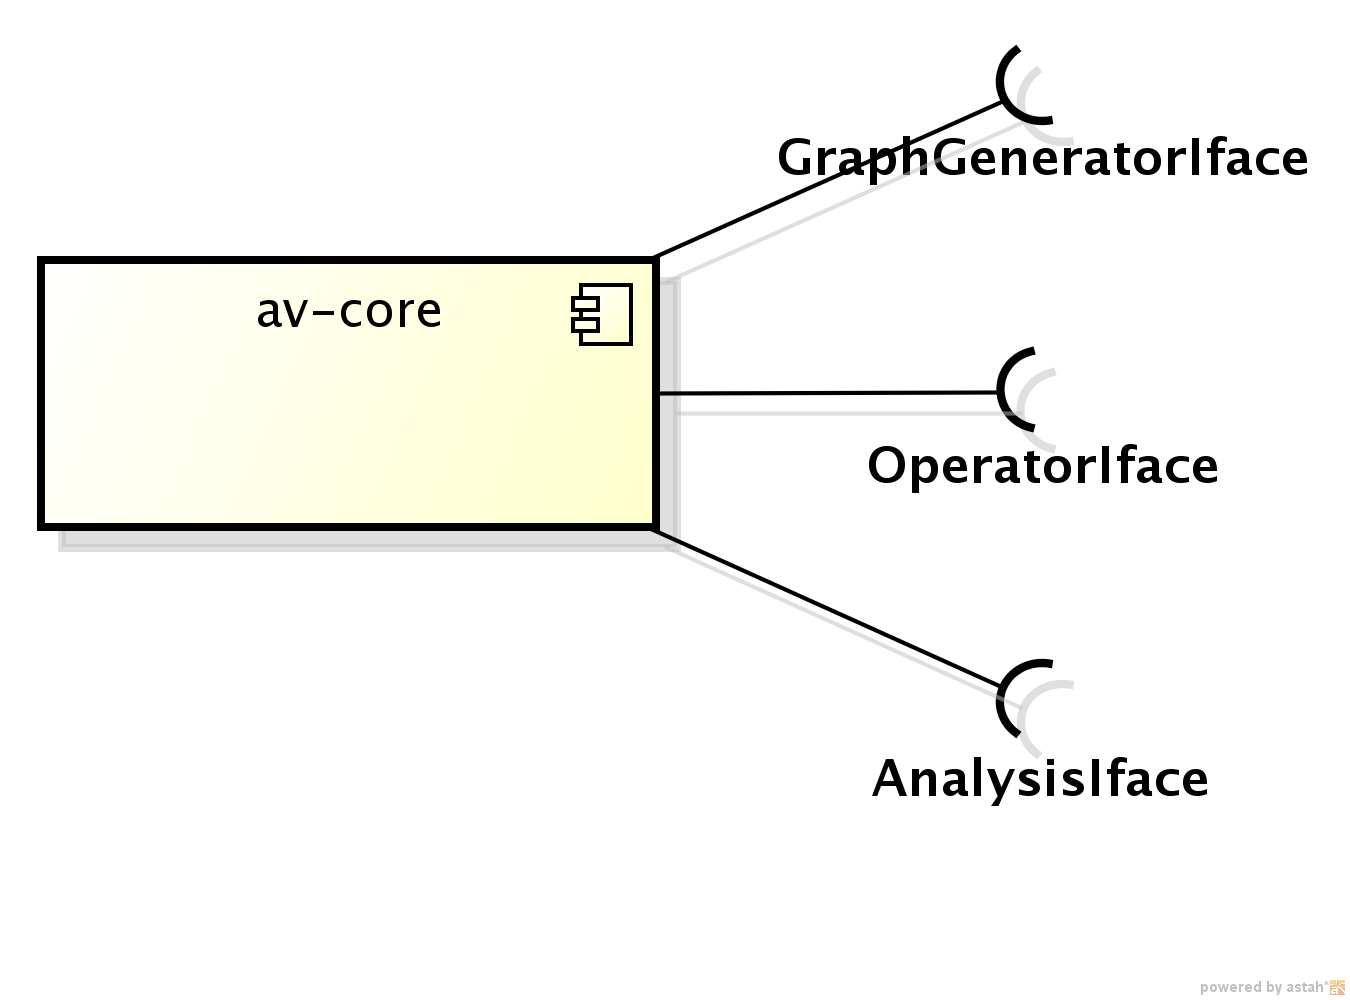
\includegraphics[width=1.0\textwidth]{./uml/archval_module_cmp.png}
  \caption{Rozdělení systému na samostatné komponenty.\label{design-modules}}
\end{figure}

Je potřeba definovat je dostatečně obecně -- interfaces (možnost oddědění vlastního rozšiřujícího rozhraní).

\subsection{Doménové objekty}

% TODO: popsat jednotlivé

\begin{itemize}
\item \emph{Graph} (class)
\item \emph{Vertex} (class)
\item \emph{Edge} (class)
\item \emph{GraphModel} -- množina grafů různých typů
\item \emph{ValidationModel} -- AST strom souboru pravidel s navázanými operátory; bude se přegenerovávat při úpravě souboru/textu v GUI, atd\ldots
\item \emph{ValidationReport}
\item \emph{AnalysisReport}
\end{itemize}

% TODO: move to appropriate position:
Třídy \emph{ValidationModel} a \emph{GraphModel} zde zavádíme zejména proto, aby bylo možné tyto objekty uložit do vhodné cache a znovu je použít. Příkladem může být případ, kdy chceme tentýž projekt (pro nějž jsme již jednou generovali graf) validovat pomocí jiné/upravené množiny pravidel nebo naopak pokud chceme použít jednu množinu pravidel pro validaci více projektů. Bylo by zbytečné opakovaně provádět náročné operace generování grafu nebo parsování souboru pravidel a navazování operátorů.

\subsection{Modul av-core}
TODO: popis validačního procesu: rozepsat
\begin{itemize}
\item systém načte moduly
\item systém zkontroluje základní předpoklady - existuje alespoň jeden modul pro generování grafu, alespoň jeden modul operátorů (nebo poskytovatel analyzerů ???) a alespoň jeden modul s poskytovatelem generátou výstupu
\item systém zparsuje soubor pravidel a vygeneruje AST
\item systém zkontroluje, zda pro AST pravidel existují potřebné providery grafů
\item systém zkontroluje, zda pro AST pravidel existují všechny operátory
\item systém provede nabindování operátoru na uzly AST pravidel
\item systém vygeneruje pro projekt všechny požadované grafy
\item systém vyhodnotí AST nad grafy pomocí operátorů, zjištěná porušení pravidel bude zapisovat do validačního reportu
\item systém projde všechny analyzátory a nechá je vygenerovat analyzační report
\item systém pomocí výstupních modulů vygeneruje reporty (na základě konfigurace ???)
\end{itemize}

Jádro systému bude poskytovat třídy a rozhraní popsané v tabulce \ref{design-archval_core_components}.

\begin{table}
  \caption{Tabulka komponent jádra systému. \label{design-archval_core_components}}
  \begin{center}
    \begin{tabular}{| l | l | p{8cm} | }
      \hline
      \textbf{Název} & \textbf{Typ} & \textbf{Zodpovědnost} \\
      \hline
      \hline
      Action & class & integrace s běhovou platformou, vstupní/aktivační bod systému \\ \hline
      ValidationTask & class & řízení procesu validace \\ \hline
      Validator & class & bude provádět validaci pravidel v grafu na základě vstupních pravidel \\ \hline
      Analyzer & class & bude provádět statistické analýzy (pro návrhové principy, které nelze popsat přesnými pravidly) \\ \hline
      ConfigurationManager & class & komponenta zprostředkující konfigurační uživatelské volby jádru programu \\ \hline
      GraphGeneratorManager & class & zinicializuje jednotlivé moduly pro generování grafů a použije je pro vygenerování grafů (pokud budou tyto grafy potřeba) \\ \hline
      ReportGeneratorManager & class & použije některé z dostupných poskytovatelů pro generování výstupu pro vygenerování reportu \\ \hline
      GraphGeneratorIface & interface & rozhraní, které musí implementovat poskytoval generátoru grafu \\ \hline
      OperatorIface & interface & rozhraní, které musí implementovat poskytovatel balíčku operátorů \\ \hline
      ReportGeneratorIface & interface & rozhraní, které musí implementovat poskystovatel modulu pro generování výstupních reportů \\ \hline
      AnalysisIface & interface & rozhraní, které musí implementovat poskytovatel analýzy nad některým z grafů \\ \hline
      GraphGeneratorRegister & class & třída poskytující přístup k informacím o existujících poskytovatelích generátorů grafu \\ \hline
      OperatorRegister & class & třída poskytující přístup k informacím o existujících poskytovatelích operátorů \\ \hline
      AnalysesRegister & class & třída poskytující přístup k informacím o existujících poskytovatelích komponent analýzy \\ \hline
      ReportGeneratorRegister & class & třída poskytující přístup k informacím o existujících poskytovatelích generátorů výstupních reportů \\ \hline
    \end{tabular}
  \end{center}

\end{table}

%% TODO: add to table of important components
%% TODO: move to part about spi
\begin{itemize}
\item \emph{PredicateInterface}
\item \emph{VertexSelectorInterface}
\item \emph{EdgeSelectorInterface}

\item \emph{GraphModelGenerator} -- updateGraphModel() -- přegeneruje graph model -- pouze doplní požadované chybějící grafy, regenerate() -- kompletně zruší všechny grafy a vyganeruje nové (všechny požadované)
\end{itemize}

Na obrázku \ref{design-archval_core} jsou zobrazeny komponenty modulu \emph{archval-core}.

TODO: připsat k rozhraní graph generator: Reprezentuje komponentu, která provede převod zdrojových kódů na graf (zobrazení, které vybraným elementům AST přiřadí množinu vrcholů $V$ grafu $G$).

\begin{figure}[h!]
  \centering
  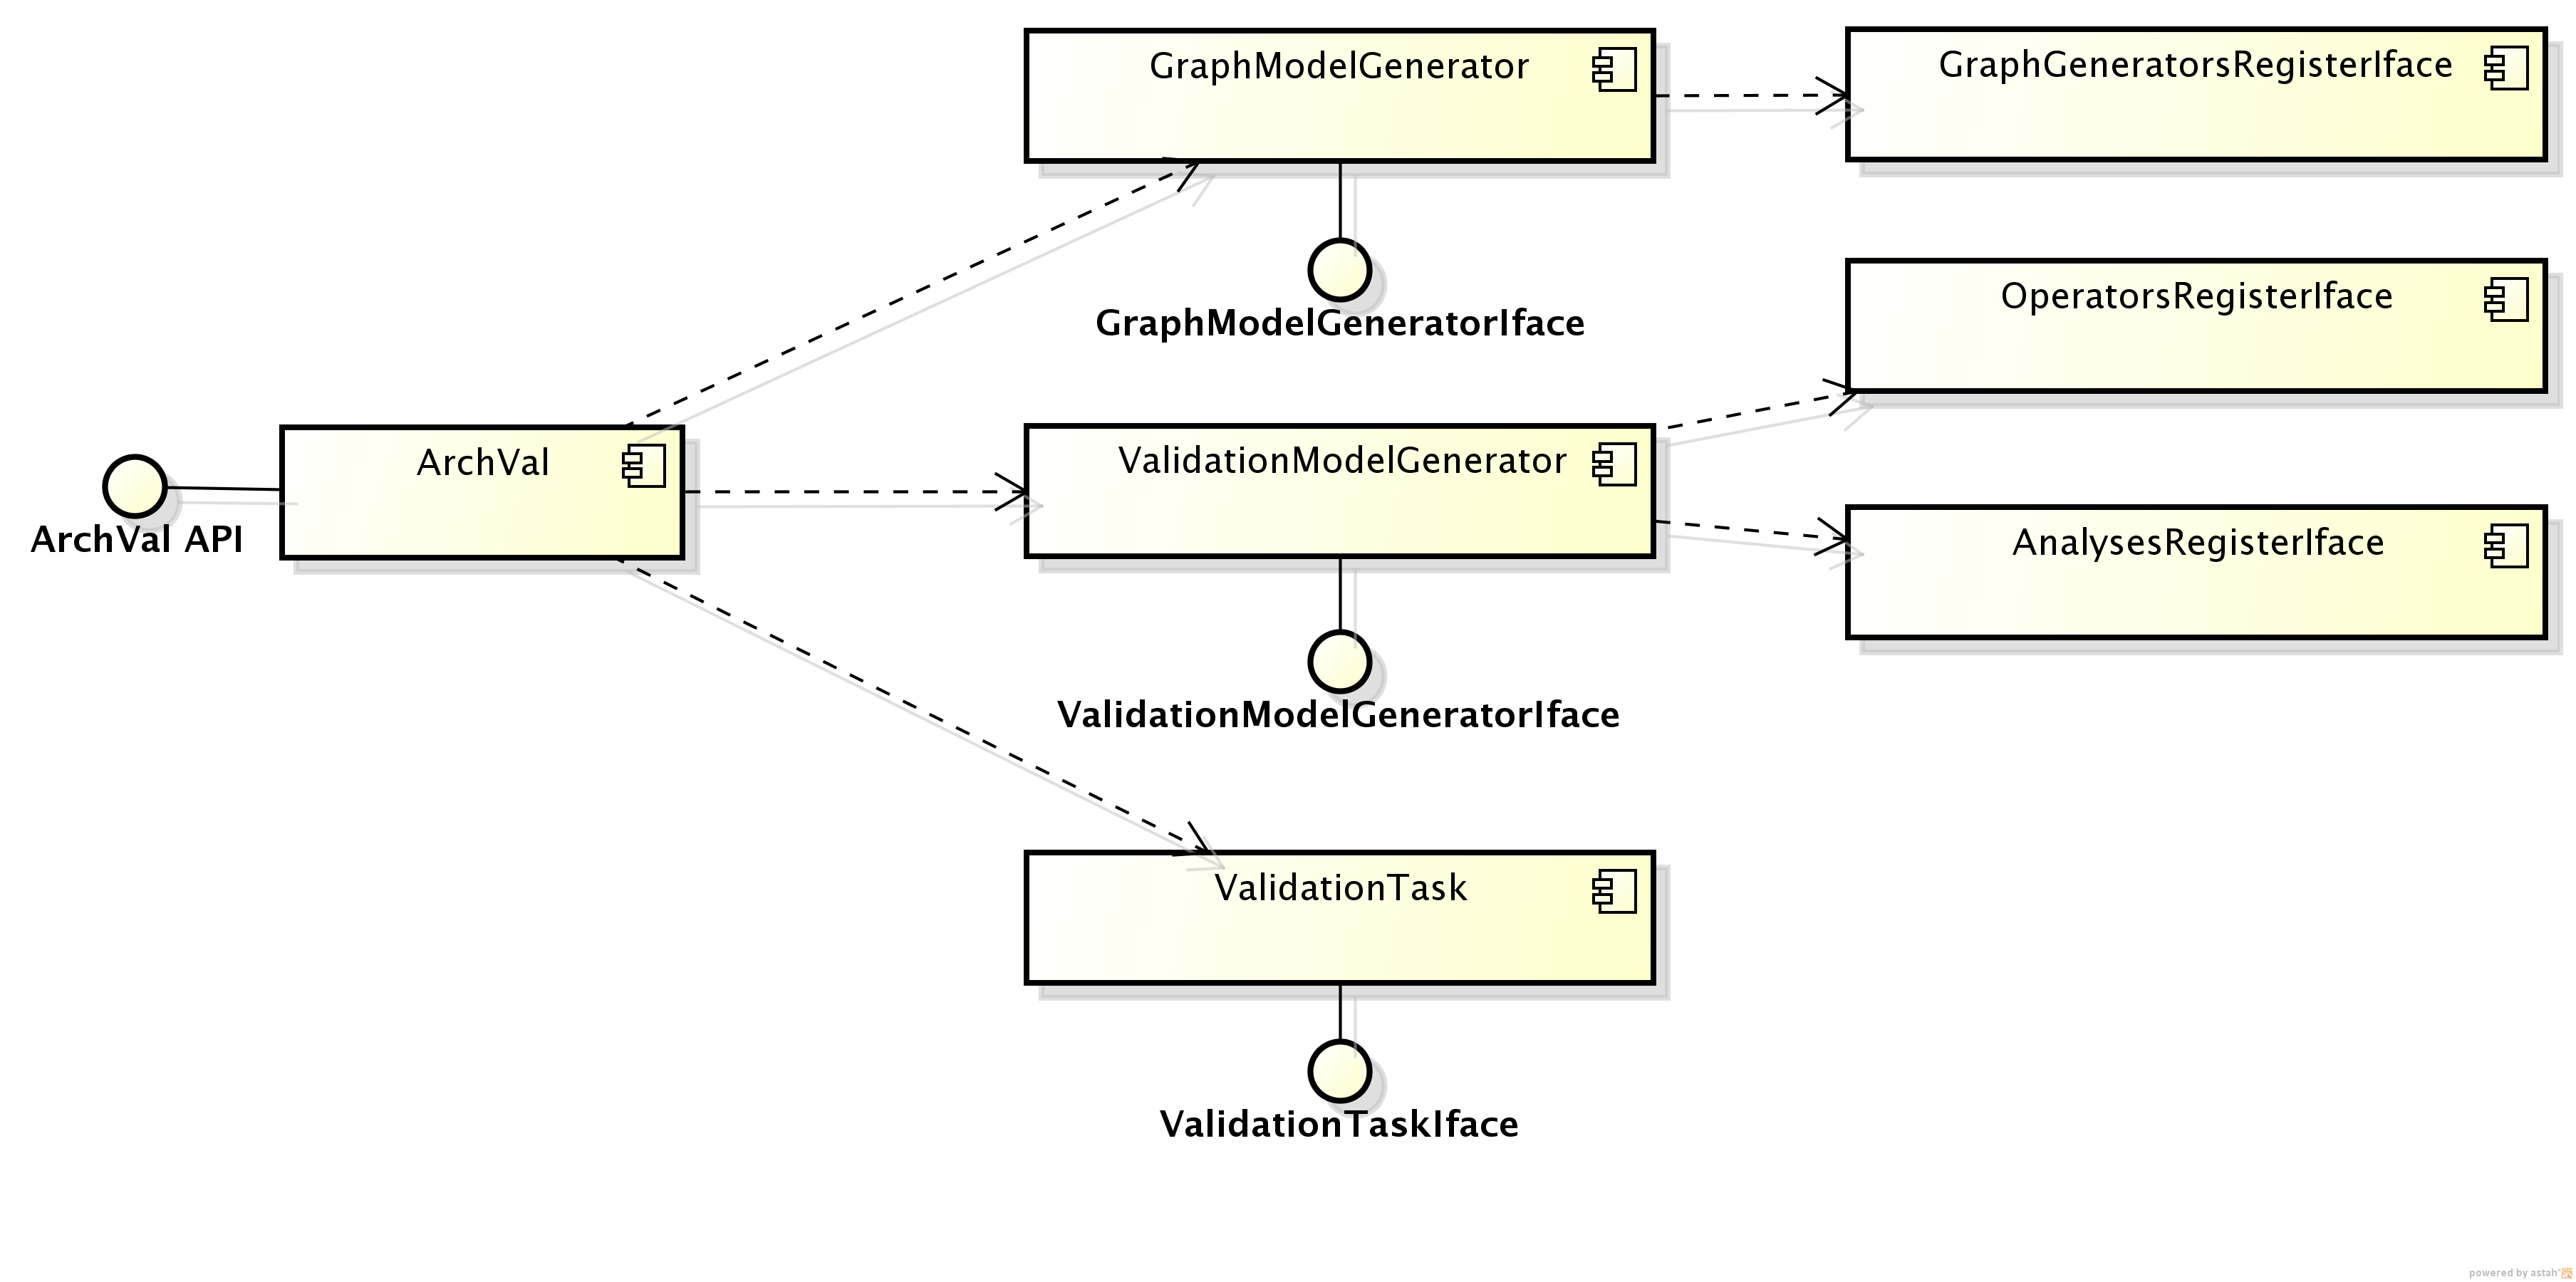
\includegraphics[width=1.0\textwidth]{./uml/archval_core_cmp.png}
  \caption{Komponenty jádra systému ArchVal.\label{design-archval_core}}
\end{figure}

TODO: přesunout do sekce popisující rozhraní \emph{GraphGeneratorInterface}:

Komponenta typu \emph{GraphGenerator} je znázorněna na obrázku \ref{design-graph_generator_io}.

\begin{figure}[h!]
  \centering
  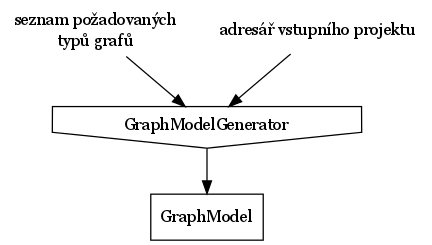
\includegraphics[width=0.45\textwidth]{./graphs/graph_generator_io_graph.png}
  \caption{Znázornění vstupů a výstupů komponenty typu \emph{GraphGenerator}.\label{design-graph_generator_io}}
\end{figure}

\subsubsection{Action}
Integrace do běhové platformy. Reprezentuje uživatelskou akci. Bude implementováno na základě zvolené implementační platformy (akce v GUI).

% TODO: rozhodnout, jestli se bude jmenovat tato komponenta Controller nebo ValidationTask
\subsubsection{Controller / ValidationTask}
Samostatné vlákno s řízením celého validačního procesu. Synchronized sekce. Vstupem bude vhodná specifikace umístění analyzovaného projektu.

TODO: vyladit následující interface
\begin{itemize}
\item setProject()
\item startValidationThread()
\item cancelValidationThread()
\item getReport()
\end{itemize}

\subsubsection{Validator}
Vstupem bude soubor pravidel

Komponenta \emph{Validator} je znázorněna na obrázku \ref{design-validator_io}.

\begin{figure}[h!]
  \centering
  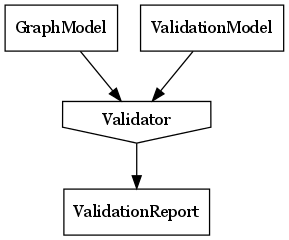
\includegraphics[width=0.45\textwidth]{./graphs/validator_io_graph.png}
  \caption{Znázornění vstupů a výstupů komponenty \emph{Validator}.\label{design-validator_io}}
\end{figure}

\begin{itemize}
\item registerOperatorPackage()
\item performValidation() : ValidationReport
\end{itemize}

Výstupem bude ValidationReport (vnitřní struktura, která se bude posléze převádět na vhodnou vnější reprezentaci).

\subsubsection{Analyzer}
TODO: analyzer providers ??? - analyzer nejspíš dostane k dispozici graf (opět musí specifikovat nad jakým grafem pracuje) a výstupem bude AnalysisReport (TBD!)

SPI -- poskytovatel služby, lookup, avd
% TODO: navrhnout aplikaci tak, aby mela vice rozhrani (nejen GUI, ale i moznost integrace, moznost textoveho vstupu pravidel)

\subsubsection{ValidationModelGenerator}
TODO: add name of this component to the table of components
TODO: add to appropriate place in the document

Znázornění vstupů a výstpů komponenty \emph{ValidationModelGenerator} je na obrázku \ref{design-validation_model_generator_io}.

% TODO: zkontrolovat, že 'výše popsaných pravidel' odkazuje na nějaká předchozí pravidla dříve v práci
Vstupem je množina pravidel zapsaná ve vhodné serializaci výše popsaných matematických pravidel.

\begin{figure}[h!]
  \centering
  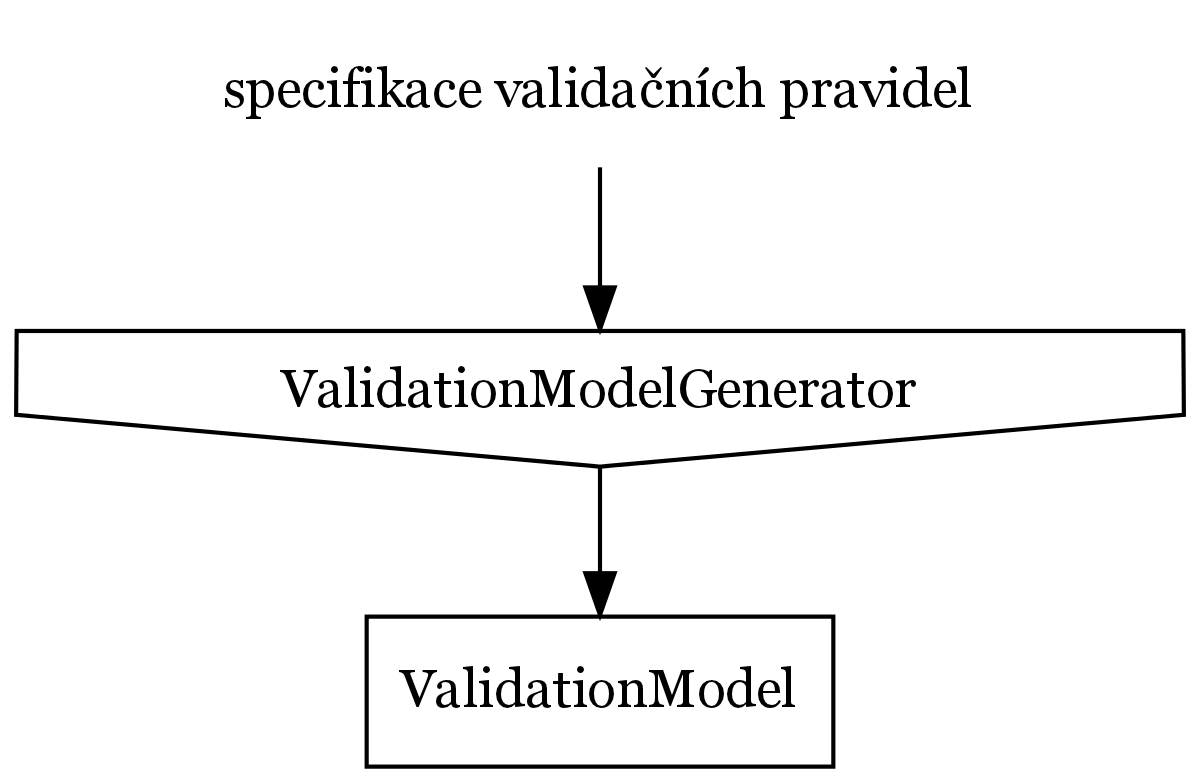
\includegraphics[width=0.5\textwidth]{./graphs/validation_model_generator_io_graph.png}
  \caption{Znázornění vstupů a výstupů komponenty \emph{ValidationModelGenerator}.\label{design-validation_model_generator_io}}
\end{figure}

Různé vstupy: File, Stream, String, \ldots

\section{Návrh rozhraní pro zadávání pravidel}
TODO: zapracovat: U každého pravidla musí být deklarace typu grafu, nad nímž má platit.
%% rozhraní pro zadávání pravidel bude dáno jazykem, který se pro definici pravidel bude používat - možná kompilátor DSL jazyka, výrazy, atd.
\begin{itemize}
\item rozhraní pro zadávání pravidel
\item formát zadávání pravidel (serializace formalismu tak, aby jej bylo možné textově nebo jinak zadávat)
\end{itemize}

\section{Návrh rozhraní pro ověřování platnosti pravidel (validaci)}
\begin{itemize}
\item výstupní rozhraní
\item validační události
\end{itemize}
% TODO: navrhnout formát výstupu

%% TODO:
% typy grafů: class hierarchy graph, call graph
% call graph: wikipedia (<<invokes>> vazby)
%
% http://en.wikipedia.org/wiki/Call_graph
%

%% TODO: dat na spravne misto
\section{Návrh technologií pro implementaci}
\begin{itemize}
\item NetBeans platform
\item Maven project
\item Java 1.6
\item vstupem bude java maven projekt
\item \ldots
  % TODO: vytvorit prehled technologii i s jejich popisy
\end{itemize}
